\section{Document Representation}
This section describes how the system design represents a text document and how this design allows the system to detect merging conflicts. The design will use a two-level granularity; the first level represents all of the paragraphs in the document, and the second level represents all of the sentences in the individual paragraphs. By having these two levels, merging conflicts can be examined on a sentence-by-sentence basis. This merging process will be described in more detail in the next section when logging and merging are addressed.
%\vspace{12 pt} \\

The design assumes that every paragraph and every sentence will have a corresponding paragraph and sentence ID. Each paragraph ID will be unique, and each sentence ID will be unique for its corresponding paragraph. This design specification will be accomplished by assigning a masked 32-bit long value to all paragraphs and sentences. The mask will be a 10-bit block corresponding to a unique User ID that will be assigned to each user when the peer-to-peer document is first created. The remaining 22 bits will be assigned when the paragraph or sentence is first created. The mask that is used corresponds to the User ID of the user that initially created the paragraph or sentence.  This masked long value is shown in Figure ~\ref{fig:id_figure} (below).
%\vspace{12 pt} \\

\begin{figure}[b]
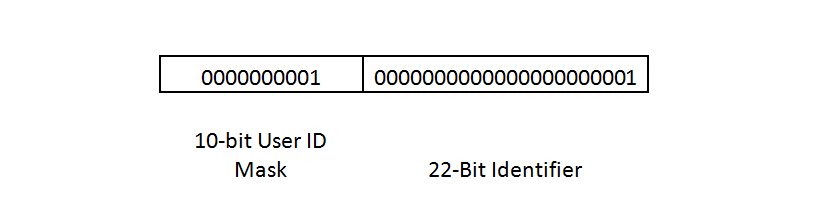
\includegraphics[scale=0.55]{Figure1.png}
\caption{Paragraph and sentence representation. The 10-bit mask is unique to each user, and the 22-bit identifier is chosen by the user's system when the paragraph or sentence is first created. The above representation represents the first item created by User 1.}
\label{fig:id_figure}
\end{figure}

The 10-bit mask ensures that every paragraph in the system has a unique ID. The 32-bit ID will be appended to the end of every paragraph in the system but will be unable to be translated by the text editor. This step ensures that the information is stored in the document but is not visible to the user. Within each paragraph, the 10-bit mask will be used to create an ID for each sentence. This 32-bit ID will be appended to the end of the sentence in the document, and just as above, the long value will not be seen by the user. A sample document is shown in Figure ~\ref{fig:file_figure} (below).
%\vspace{12 pt} \\

\begin{figure}[b]
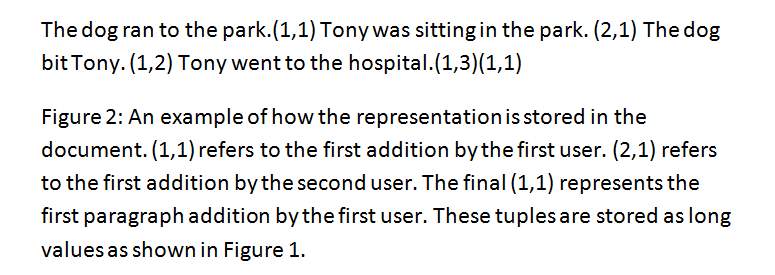
\includegraphics[scale=0.55]{Figure2.png}
\caption{An example of how the representation is stored in the document. (1,1) refers to the first addition by the first user. (2,1) refers to the first addition by the second user. The final (1,1) represents the first paragraph addition by the first user. These tuples are stored as long values shown in Figure ~\ref{fig:id_figure}.}
\label{fig:file_figure}
\end{figure}

The user will never see a document similar to this one because the 32-bit long values will not appear in the actual document, but Figure ~\ref{fig:file_figure} shows how these IDs will be stored. As you can see, the last sentence has 64 bits appended to it; one for the sentence ID, and one for the paragraph ID.  Finally, the ID of a paragraph or sentence is immutable; it will never change throughout the life of the document.
%\vspace{12 pt} \\

Through this design, a paragraph knows what user it belongs to and its current collection of sentences. A sentence also knows what user it belongs to and can determine its parent paragraph by reading the last appended long value. This information will help the system merge modifications and discover any conflicts that arise due to multi-peer editing.
